\documentclass[a4j,dvipdfmx,titlepage]{article}
%Format   -----------------------
\usepackage[utf8]{inputenc}
\usepackage[euler]{textgreek}
\usepackage{enumitem}
\usepackage[margin=30mm]{geometry}
\usepackage{comment}
\usepackage{url}
\usepackage{float}
\usepackage{subcaption}
\usepackage{textcomp}
\usepackage{palatino}
\usepackage{xparse}
%Format   -----------------------

%Circuit ------------------------
%\begin{comment}
\usepackage{amsmath,amssymb}
\usepackage[dvipdfmx]{graphicx}
\usepackage{siunitx}
\usepackage{tikz}
\usepackage{circuitikz}
%\end{comment}
%Circuit ------------------------

%Command ---–--------------------
\renewcommand{\figurename}{図}
\renewcommand{\tablename}{表}
%--------------------------------

%Title   ------------------------
\begin{titlepage}
    \title{実験レポートA1}
    \author{東京大学工学部電気電子工学科 03210517\\藤田 誠之\\~\\ 共同実験者  河野亮介・梶谷優貴・パリナヨックサタユ}
    \date{May 15, 2021}
\end{titlepage}
%Title   ------------------------
\renewcommand{\baselinestretch}{1.2}

\begin{document}

\tikzset{component/.style={draw,thick,circle,fill=white,minimum size =0.75cm,inner sep=0pt}}

\maketitle
\newpage

\section{実験目的}
この実験を通し、ディジタル回路の特性の理解と、物理的にディジタル回路を構成する技術の理解をすることを目的とする。

\section{考察課題}

\begin{enumerate}[label={(\arabic*)}]
  \item 測定レンジと内部抵抗にはどのような関係があるのか、図A1.13を参照しながら推測し、測定結果と比較してみよ。pn接合ダイオードの電流電圧特性が正確に測定されていると思われる領域と、測定系の限界が(補正をしても)測定結果に影響を与えられていると思われる領域を明らかにせよ。
\end{enumerate}
内部抵抗の補正をせずに、図の回路図を組んで計測した値をグラフ化し、低電圧時の部分を拡大すると、以下のようになる。
\begin{figure}[H]
  \begin{center}
  \includegraphics[width=12cm]{../graph/figures/data_pn_a_normal_big_before.png}
  \caption{$I_D$-$V_{DS}$グラフ(内部抵抗による補正前) 拡大}
  \end{center}
\end{figure}

0.3V付近で大きく測定値が動いていることがわかる。これは、0.3V付近で、使用した電圧計のマイナス端子を最大電圧0.3Vから最大電圧1.0Vのものへ切り替えたからと推測できる。ここで、最大電圧0.3Vの端子につなげたときの電圧計の内部抵抗は$2.98\Omega$、1.0Vのときは$9.97\Omega$である。電流の値を以下の式で補正した。
$$
I_{corrected} = I_{observed} - \frac{V}{r}
$$
その結果をグラフにすると以下のようになった。

\begin{figure}[H]
  \begin{center}
  \includegraphics[width=12cm]{../graph/figures/data_pn_a_normal.png}
  \caption{$I_D$-$V_{DS}$グラフ(内部抵抗による補正後) 拡大}
  \end{center}
\end{figure}

このように、予想されるように曲線がつながった。しかし、このような計算の結果、一部の電流値がマイナスとなった。これは測定誤差に起因するものと思われる。また、図のように対数グラフを作成する際、0.2以下の部分は測定器の限界によってデータが散乱しており、$R^2$の値を計算しても0.30と相関があるとは言えない。この付近のデータは順バイアスの再結合などの特性を調べるために重要であるが、測定系の限界になってしまっている。

\begin{enumerate}[label={(\arabic*)}]
    \setcounter{enumi}{1}
    \item pn接合ダイオードの電流電圧特性について、測定結果と理論を定量的に比較し、理論からのズレとその要因を考察せよ。
\end{enumerate}

FETトランジスタを以下の回路図のようにつなげ、電圧と電流を測定した。Dは接続していない。このように接続すると、トランジスタはpn接合ダイオードとなる。

\begin{figure}[H]
  \begin{center}
    \begin{circuitikz}[american currents]
     \ctikzset{american inductors}
	  \draw (0,4)
      to[battery1] (0,0)
      to[short] (5,0)
	  to[short] (5,2) 
	  node[component]{V}
	  to[short] (5,4)
	  to[short] (2.5,4) node[component]{A} to [short] (0,4);
	  \draw(5,4)
	  to[short] (6,4);
    \draw(7,2)
	  node[njfet](njfet){}
	  (njfet.base) node[anchor=east] {G}
	  (njfet.collector) node[anchor=south] {D}
	  (njfet.emitter) node[anchor=west] {S};
	  to[short] (3,0);
	  \draw(6,4)
	  to[short] (njfet.base);
    \draw(4,0)
    to[short] (7,0)
    to[short] (njfet.emitter);
	  \draw ($(njfet)-(0.18,0)$) circle [radius=18pt];
    \end{circuitikz}
    \caption{実験の回路図}
  \end{center}
\end{figure}
ここで、電圧計で計測される電圧は$V_{GS}$、電流計で計測される電流を$I$とし計測されたデータをグラフ化したものが以下である。

\begin{figure}[H]
\begin{center}
\includegraphics[width=12cm]{../graph/figures/data_pn_a_normal.png}
\caption{$I_D$-$V_{DS}$グラフ}
\end{center}
\end{figure}

PN接合の特性は一般に以下の式で示される。
$$
I = I_0\left(e^{\frac{qV}{kT}}-1\right)
$$
しかし、実際のPN接合ダイオードでは、結晶欠陥や寄生抵抗などが存在することから、理想的な状態とはかなり異なっている。順バイアス時には、電圧を上げていくに連れ、まず欠陥による再結合により、電流が$e^{\frac{qV}{2kT}}$に比例するようになる。その後、$e^{\frac{qV}{kT}}$に比例した後、高注入効果により再び$e^{\frac{qV}{kT}}$に比例し、最終的には寄生抵抗により電圧と比例関係となるようになる。\\

電流の対数をとったものの図は以下のようになる。
\begin{figure}[H]
  \begin{center}
  \includegraphics[width=12cm]{../graph/figures/data_pn_a_normal_log.png}
  \caption{$I_D$-$V_{GS}$対数グラフ}
  \end{center}
\end{figure}
ここで、青の点の部分はおよそ電流が$e^{\frac{qV}{kT}}$に比例していると考えられる。青い部分の傾きの逆数を最小2乗法で求めると、0.030となった。室温を$\deg{20}$とすると${qV}{kT}=0.026$となるので、誤差率11\%とよく一致していることがわかる。また、赤い部分は電流がおおよそ$e^{\frac{qV}{kT}}$に比例すると考えられるが、この部分の傾きを同じく最小二乗法で計算すると0.13となる。赤の部分に関しては高注入効果及び寄生抵抗により傾きがだんだんと減少し0に収束していくはずであるので、得られた実験結果は理論と一致しているということができる。また、逆バイアス時については、電流の対数の値が一定の値に収束している、つまり電流が電圧に比例するようになっていることがわかる。このときの電流の対数の収束値は-8.92であるため、電流は電圧に比例定数$e^{-8.62}=5431$で比例していることがわかる。このことから、電流が内部抵抗に流れているとすると内部抵抗の大きさが$5431\Omega$ということが推測できる。実際の内部抵抗の大きさは$2980\Omega$であるため、誤差率が82\%程度となっているが、生成などによりこの抵抗値の計算される値が大きくなったと考えられる。また、高逆バイアスによる降伏は起こっていないこともわかる。

\begin{enumerate}[label={(\arabic*)}]
  \setcounter{enumi}{2}
  \item FETの静特性について理論を調べ、測定値と理論値を定量的に比較した上で、理論からのズレを考察せよ。
\end{enumerate}

pn接合ダイオードの電流電圧特性は、\\
\begin{center}[H]
  三極管領域において
\end{center}
$$
I_D = \mu_nC_{OX}\frac{W}{L}\left((V_{GS}-V_{TH})V_{DS} - \frac{1}{2}V_{DS}^2\right) = \beta\left((V_{GS}-V_{TH})V_{DS} - \frac{1}{2}V_{DS}^2\right)
$$
\begin{center}[H]
    飽和領域において
\end{center}
$$
I_D = \frac{1}{2}\mu_nC_{OX}\frac{W}{L}\left(V_{GS}-V_{TH}\right)^2 = \frac{1}{2}\beta(V_{GS}-V_{TH})^2
$$
\begin{align}[H]
  \mu_n &: \mbox{電子の移動度[m}^2\mbox{/Vs]}\nonumber \\
  C_{OX} &: \mbox{単位面積あたりの酸化膜容量[F/m}^2\mbox{]} \nonumber \\
  W &: \mbox{チャネル幅[m]} \nonumber \\
  L &: \mbox{実効チャネル長[m]} \nonumber \\
  \beta &: \mbox{利得係数} \nonumber
\end{align}
と表すことができる。ここで、今回使用したトランジスタ2SK30ATMのゲート・ドレイン間しゃ断電圧$V_{TH}$($V_{GS(OFF)}$)は規格書によると下限が-0.4V、上限が-5.0Vとなっている。図の回路図のような回路を組み立て、$V_{DS}$を変化させながら$I_D$を測定した結果、得られたデータは図のようになった。

\begin{figure}[H]
  \begin{center}
    \begin{circuitikz}[american currents]
     \ctikzset{american inductors}
    \draw (0,0)
    to[battery1] (0,2)
    to[short] (1,2)
    to[short] (1,1) node[component](v2){V}
    to[short] (1,0)
    to[short] (0,0);
    \draw ($(v2)+(0.4,0)$) node[anchor=west] {$V_{GS}$};
    \draw(4,2.27) node[njfet](njfet){}
    (njfet.base) node[anchor=north] {G}
    (njfet.collector) node[anchor=east] {D}
    (njfet.emitter) node[anchor=east] {S};
    \draw ($(njfet)-(0.18,0)$) circle [radius=18pt];
    \draw (0,2)
    to[short] (njfet.base);
    \draw (1,0)
    to[short] (4,0)
    to[short] (njfet.emitter);
    \draw (njfet.collector)
    to[short] (4,4)
    to[short] (5,4)
    to[short] (5,2)
    node[component](v1){V}
    to[short] (5,0)
    to[short] (4,0);
    \draw ($(v1)+(0.4,0)$) node[anchor=west] {$V_{DS}$};
    \draw (5,4)
    to[short] (6,4)
    node[component]{A}
    to[short] (7,4)
    to[battery1] (7,0)
    to[short] (4,0);
    \end{circuitikz}
    \caption{実験の回路図}
  \end{center}
\end{figure}

\begin{figure}[H]
  \begin{center}
  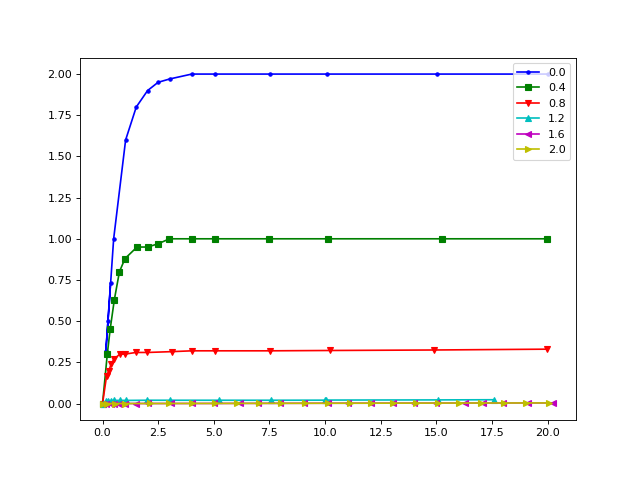
\includegraphics[width=12cm]{../graph/figures/all.png}
  \caption{$I_D$-$V_{DS}$グラフ}
  \end{center}
\end{figure}

\begin{figure}[H]
  \begin{center}
  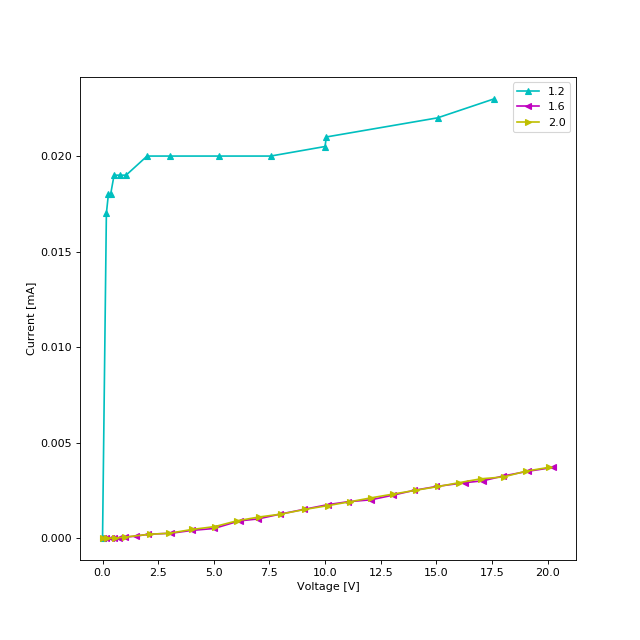
\includegraphics[width=12cm]{../graph/figures/lower.png}
  \caption{$I_D$-$V_{DS}$グラフ(下部分拡大)}
  \end{center}
\end{figure}

上記に記した$I_D$の式を用いて、計測結果をフィッティングしようと試みた。$\beta$と$V_{TH}$は理論上$V_{DS}$に関係することのない定数であるとして、まずは飽和領域での値を合わせようとした。\\
フィッティングした結果、$\beta = 2.25, V_{TH} = -1.335$とし、得られた飽和時のドレイン電流は以下の通りである。

\begin{table}[H]
  \begin{center}
    \begin{tabular}{|c|c|c|c|} \hline
      $V_{GS}$[V] & \begin{tabular}{c}$I_D$の飽和時の\\ドレイン電流[mA]\end{tabular}& \begin{tabular}{c}フィッテイング曲線の$I_D$の\\飽和時のドレイン電流[mA]\end{tabular}& 誤差率 \\ \hline
      0.0 & 2.00 & 2.00 & 0.0\% \\ \hline
      -0.4 & 1.00 & 0.984 & 98\% \\ \hline
      -0.8 & 0.33 & 0.322 & 98\% \\ \hline
      -1.2 & 0.023 & 0.021 & 91\% \\ \hline
      \end{tabular}
      \caption{飽和領域の$I_D$の誤差率}
  \end{center}
\end{table}

このように、飽和時のドレイン電流については非常によくフィッティングすることができた。ただ、$V_{TH}=-1.335$としているため、$V_{GS} < -1.335\mbox{V}$となるデータについてはトランジスタがONとなっていないため、上記の式では表せない。これについても、読み取られたデータと合致している。つまり、$V_{GS}$が$V_{TH}$を下回っている$V_{GS} = 1.6, 2.0$については、三極管領域が存在せず、直線でフィッティングできることがわかる。\\
ただし、このフィッティング曲線はピンチオフ電圧の誤差が大きいこともわかる。理論上、ピンチオフ電圧は$V_{p} = V_{GS}-V{TH} = V_{GS} + 1.335$となる。それぞれの$V_{GS}$についての誤差は以下の表の様になる。

\begin{table}[H]
  \begin{center}
    \begin{tabular}{|c|c|c|c|} \hline
      $V_{GS}$[V] & \begin{tabular}{c}データから読み取れた$V_p$\end{tabular} & \begin{tabular}{c}フィッテイング曲線の$V_p$\end{tabular}& 誤差率 \\ \hline
      0.0 & 3.0 & 1.335 & 56\% \\ \hline
      -0.4 & 1.5 & 0.955 & 36\% \\ \hline
      -0.8 & 0.8 & 0.555 & 30\% \\ \hline
      -1.2 & 0.2 & 0.155 & 22\% \\ \hline
      \end{tabular}
      \caption{$V_p$の実験値と理論値の誤差}
  \end{center}
\end{table}

このように、とても誤差が大きくなってしまっていることがわかる。ここで、$V_{P} = V_{DS} - V_{TH}$であるから、$V_{TH}$が実際の値よりも大きく測定されたか、$V_{GS}$が実際の値よりも小さく測定されたということが考えられる。$V_{GS}$は直接電圧計を当てて測定しているため、大きな誤差が生じるとは考えにくいため、フィッティングした際に計算された$V_{TH}$の値に大きな誤差があると考えられるが、他のパラメータはよくフィッティングできているため、どうしてこのような結果となったのかをこのレポートの提出までに原因を特定することはできなかった。

\section{参考文献}
「MOSFET 電気的特性(静的特性)について」\url{https://toshiba.semicon-storage.com/jp/semiconductor/knowledge/faq/mosfet/electrical-characteristics-of-mosfetsst}\\\url{atic-characteristics-vth.html} 2021年5月1日アクセス\\~\\
「What is the pinch off voltage for a JFET?」\url{http://electrotopic.com/what-is-the-pinch}\\\url{-off-voltage-for-a-jfet/} 2021年5月1日アクセス\\~\\
「MOSFETの構造と動作原理」 \url{https://www.shindengen.co.jp/products/semi/column/basic/mosfet/mosfet_1.html} 2021年5月1日アクセス\\
竹中充先生講義「半導体デバイス工学」2021年5月10日付 配布資料No.1, No.2, No.3より\\~\\
黒田忠広先生講義「電子回路I」2021年5月10日付 配布資料 第1回, 第2回
\end{document}


\begin{comment}
--------------------------------
--見出し
\section{実験方法}
--番号を振る
\begin{enumerate}[label={(\arabic*)}]
\item
--画像の挿入
\begin{figure}[H]
\begin{center}
\includegraphics[width=8cm]{figures/name}
\caption{title)}
\end{center}
\end{figure}

--回路(例)
\begin{figure}[H]
\begin{center}
\begin{circuitikz}[american currents]
\ctikzset{american inductors}
\draw (0,0)
to[sV=V_s$] (0,2)
to[L=L_2$] (6,2)
to[C=$$
to[european resistor=\Omega$] (6,0)
to[short] (3,0);
\end{circuitikz}
\caption{3次規格化0-R型LPF}
\end{center}
\end{figure}

--表
\begin{table}[H]
\begin{center}
\begin{tabular}{|l|l|c||} \hline
11 & 12 & 13 \ \hline
21 & 22 & 23 \ \hline
31 & 32 & 33\ \hline
\end{tabular}
\caption{title}
\end{center}
\end{table}
\end{comment}